
\documentclass{article} % For LaTeX2e
\usepackage{iclr2025_conference,times}

% Optional math commands from https://github.com/goodfeli/dlbook_notation.
\input{math_commands.tex}

\usepackage{hyperref}
\usepackage{url}
\usepackage{graphicx}
\usepackage{booktabs}
\usepackage{float}

\title{Design and Implementation of a Multi-layer Memory System \\ for Large Language Models}

% Authors must not appear in the submitted version. They should be hidden
% as long as the \iclrfinalcopy macro remains commented out below.
% Non-anonymous submissions will be rejected without review.

\author{Anonymous}

% The \author macro works with any number of authors. Use \And and \AND to separate authors.

\newcommand{\fix}{\marginpar{FIX}}
\newcommand{\new}{\marginpar{NEW}}

%\iclrfinalcopy % Uncomment for camera-ready version, but NOT for submission.
\begin{document}


\maketitle

\begin{abstract}
Large Language Models (LLMs) are inherently stateless systems that generate independent responses without retaining information from previous interactions. This limitation leads to repetitive user inputs, inability to personalize responses, and failure to learn from past mistakes. This paper presents a multi-layer memory system designed to address these challenges through three complementary mechanisms: (1) a token-based context window for recent context retention, (2) a conversation summary module for mid-term memory compression, and (3) a dynamic cheatsheet (Insights) for long-term knowledge extraction and retrieval. The system is evaluated through comparison experiments and ablation studies. Results demonstrate that the full memory system achieves a 73.3\% keyword recall rate compared to 33.3\% for the baseline, representing a 40\% improvement in long-term memory retention. The ablation study reveals that conversation summary is the most critical component, while insights provide additional benefits for specific knowledge retrieval.
\end{abstract}

\section{Introduction}
\label{sec:intro}

Large Language Models (LLMs) have demonstrated remarkable capabilities across a wide range of natural language processing tasks. However, these models are fundamentally \textbf{stateless systems}---each prompt is processed independently without any inherent mechanism to retain information from previous interactions.

This stateless nature leads to several practical limitations in conversational applications:

\begin{itemize}
    \item \textbf{Repetitive Information}: Users must repeatedly provide the same background information across sessions.
    \item \textbf{Lack of Personalization}: The model cannot adapt responses based on user preferences or historical behavior.
    \item \textbf{Inability to Learn from Feedback}: Corrections provided in previous interactions are forgotten, leading to repeated mistakes.
\end{itemize}

While various approaches have been proposed to address these limitations, including context concatenation, retrieval-augmented generation (RAG), and memory compression techniques, each comes with its own trade-offs between memory capacity, retrieval accuracy, and computational efficiency.

This paper presents a \textbf{multi-layer memory system} that combines three complementary mechanisms:

\begin{enumerate}
    \item \textbf{Token-based Context Window}: Maintains recent conversation history within a fixed token budget using FIFO eviction.
    \item \textbf{Conversation Summary}: Compresses older conversations into concise summaries to preserve essential information.
    \item \textbf{Dynamic Cheatsheet (Insights)}: Extracts and stores key knowledge points for long-term retention and semantic retrieval.
\end{enumerate}

The main contributions of this paper are:
\begin{itemize}
    \item A hierarchical memory architecture addressing short-term, mid-term, and long-term memory requirements.
    \item Comprehensive evaluation through comparison experiments and ablation studies demonstrating significant improvements in memory retention.
\end{itemize}

\section{Related Work}
\label{sec:related}

Memory mechanisms for language models can be broadly categorized into four types: context memory, external memory, hidden state memory, and parametric memory. This section reviews each approach and positions the proposed method within this landscape.

\subsection{Context Memory}

The most straightforward approach to providing memory for LLMs is through context concatenation, where previous conversation history is directly appended to the current prompt. This method leverages the model's native ability to process sequential information within its context window. However, as conversations grow longer, this approach faces fundamental limitations due to the fixed context window size of transformer-based models. When the accumulated context exceeds the maximum token limit, older information must be discarded, typically following a First-In-First-Out (FIFO) policy. While simple truncation ensures the model can always process the input, it inevitably loses potentially important information from earlier in the conversation. More sophisticated approaches attempt to compress older context through summarization before truncation, preserving semantic content while reducing token count.

\subsection{External Memory}

External memory systems store information outside the model's context window and retrieve relevant content at inference time. The most prevalent approach in this category is Retrieval-Augmented Generation (RAG), which uses vector databases to store and retrieve semantically similar content based on embedding similarity. RAG has proven effective for incorporating large knowledge bases into LLM responses, but its effectiveness depends heavily on the quality of retrieval and the relevance of retrieved content to the current query.

An alternative external memory approach is the Dynamic Cheatsheet method proposed by \citet{banerjee2024dynamic}. Unlike RAG, which retrieves from a static knowledge base, Dynamic Cheatsheet maintains an adaptive memory that evolves during test time. The system extracts reusable knowledge, such as solution strategies and code snippets, from previous interactions and stores them in a curated memory. When processing new queries, relevant entries are retrieved and synthesized into the context. Experimental results demonstrate significant improvements: GPT-4o's accuracy on Game of 24 increased from 10\% to 99\% using this approach, as the model learned to store and reuse a Python-based solution strategy. The key insight is that selective memory curation outperforms simple full-history appending, which can overwhelm the context window and dilute crucial information.

\subsection{Hidden State Memory}

Recurrent Neural Networks (RNNs) and their variants, such as LSTM and GRU, represent an earlier paradigm of sequence modeling with implicit memory. These architectures maintain hidden states that are updated at each time step, theoretically allowing information to persist across arbitrary sequence lengths. However, in practice, vanilla RNNs suffer from vanishing gradients that limit their effective memory span. While gating mechanisms in LSTMs and GRUs partially address this issue, the fixed-size hidden state fundamentally constrains the amount of information that can be retained. Modern transformer-based LLMs have largely superseded RNNs for language tasks, trading sequential processing for parallel attention mechanisms that better capture long-range dependencies within their context windows.

\subsection{Parametric Memory}

Recent research has explored incorporating memory directly into model parameters. Titans \citep{behrouz2024titans} introduces a neural long-term memory module that learns to memorize at test time. The architecture combines three components: persistent memory (learnable parameters encoding task knowledge), contextual memory (sliding window attention for short-term context), and a neural memory module that updates its weights during inference to store information from the input sequence. The key innovation is treating memory as a meta-learning process, where the model learns which information to store based on a "surprise" metric. Experimental results show that Titans outperform both pure transformers and modern linear recurrent models on long-context tasks, achieving effective context lengths beyond 2 million tokens. However, this approach requires architectural modifications and is not directly applicable to existing LLM APIs.

\subsection{Comparison of Memory Approaches}

Table~\ref{tab:memory_comparison} summarizes the characteristics and applicable scenarios of each memory approach discussed above.

\begin{table}[H]
\caption{Comparison of memory approaches for LLMs}
\label{tab:memory_comparison}
\begin{center}
\begin{tabular}{p{2.5cm}p{3cm}p{3cm}p{3cm}}
\toprule
\textbf{Approach} & \textbf{Applicable Scenarios} & \textbf{Advantages} & \textbf{Limitations} \\
\midrule
Context Memory & Short conversations, real-time interaction & Simple, no extra storage & Limited by context window \\
External Memory (RAG) & Large-scale knowledge retrieval & Scalable, rich knowledge & Retrieval quality dependent \\
External Memory (Cheatsheet) & Long conversations, learning tasks & Adaptive, knowledge accumulation & Requires curation mechanism \\
Hidden State (RNN) & Sequential modeling (outdated) & Theoretically unlimited & Vanishing gradients, limited capacity \\
Parametric Memory & Ultra-long context ({>}2M tokens) & Powerful memorization & Requires model modification \\
\bottomrule
\end{tabular}
\end{center}
\end{table}

\subsection{Positioning of This Work}

This work combines external memory with context-based approaches to provide comprehensive memory coverage without requiring model modifications. The system employs three complementary mechanisms targeting different temporal scales: a token-based context window for short-term memory (recent conversation turns), conversation summarization for mid-term memory (compressed session history), and a Dynamic Cheatsheet-inspired Insights module for long-term memory (persistent knowledge across sessions). This layered architecture allows the system to work with any LLM through standard API calls.

\section{Method}
\label{sec:method}

The proposed multi-layer memory system consists of three complementary components that address different temporal scales of memory retention: a token-based context window for short-term memory, conversation summarization for mid-term memory, and a dynamic cheatsheet (Insights) for long-term memory. Figure~\ref{fig:architecture} provides an overview of the system architecture.

To ensure portability across different LLMs, all token budgets are defined as proportions of the model's context window $C$ rather than fixed values. Table~\ref{tab:token_allocation} shows the token allocation strategy used in this work.

\begin{table}[H]
\caption{Token allocation as proportions of model context window $C$}
\label{tab:token_allocation}
\begin{center}
\begin{tabular}{lcc}
\toprule
\textbf{Component} & \textbf{Ratio} & \textbf{Value (128k model)} \\
\midrule
Context Window ($T_{max}$) & 62.5\% & 80,000 tokens \\
Insights Retrieval Budget & 2.5\% & 3,200 tokens \\
Chat Response Limit & 1.5\% & 1,920 tokens \\
Summary/Curator Response & 2.5\% & 3,200 tokens \\
\midrule
Summarization Trigger & 80\% of $T_{max}$ & 64,000 tokens \\
Eviction Ratio & 50\% & oldest half \\
\bottomrule
\end{tabular}
\end{center}
\end{table}

\subsection{Context Window (Short-term Memory)}
\label{sec:context_window}

The context window serves as the foundation of the memory system, maintaining recent conversation history within a fixed token budget $T_{max}$. Given a sequence of messages $M = \{m_1, m_2, ..., m_n\}$ where each message $m_i$ has an associated token count $t_i$, the context window selects the most recent messages that fit within the budget:

$$W = \{m_k, m_{k+1}, ..., m_n\} \text{ where } \sum_{i=k}^{n} t_i \leq T_{max}$$

The algorithm processes messages from newest to oldest, accumulating tokens until the limit is reached. This FIFO (First-In-First-Out) selection policy ensures that recent context is always included in the prompt while older messages are excluded. As shown in Table~\ref{tab:token_allocation}, $T_{max}$ is set to 62.5\% of the model's context window, which for a 128k-token model yields 80,000 tokens---sufficient to accommodate extensive conversation history.

\subsection{Conversation Summary (Mid-term Memory)}
\label{sec:summary}

When the context window approaches capacity, the summary module compresses older conversations into concise summaries. The compression is triggered when accumulated tokens exceed a threshold $T_{trigger}$:

$$\text{Summary}_{new} = \text{LLM}(\text{Summary}_{old} \oplus M_{evicted})$$

where $\oplus$ denotes concatenation and $M_{evicted}$ represents the messages being removed from the context window. The LLM is prompted to identify and preserve key information including user preferences, important decisions, and contextual facts. The generated summary is prepended to subsequent prompts, providing compressed historical context without consuming excessive tokens.

\subsection{Dynamic Cheatsheet (Long-term Memory)}
\label{sec:dynamic_cheatsheet}

The Insights module implements long-term memory inspired by the Dynamic Cheatsheet approach proposed by \citet{banerjee2024dynamic}. While the original work focuses on accumulating solution strategies for specific tasks, this paper adapts the concept for general conversational memory by extracting, managing, and retrieving reusable knowledge from conversations. Unlike the summary which provides a compressed narrative, Insights capture discrete knowledge points (strategies, concepts, decisions, preferences) that persist across sessions.

\textbf{Extraction Mechanism.} After each conversation turn, a Curator model analyzes the recent dialogue (last 20 messages as context) to extract reusable knowledge. Each insight includes: textual content, category type (strategy, code, decision, concept, method), importance score (0-1), and a vector embedding for semantic retrieval. Only high-quality knowledge with importance $> 0.5$ is retained.

\textbf{Two-Stage Deduplication and Conflict Detection.} To minimize redundant API calls, the system employs a two-stage detection mechanism. In the first stage, cosine similarity is computed between the new insight embedding and all existing insights of the same type. Items with similarity $\geq 0.80$ are flagged as potentially conflicting. If no high-similarity items exist, the new insight is added directly. Otherwise, the second stage performs a batch LLM call to determine the relationship for all flagged pairs: \textit{conflict} (replace old with new), \textit{duplicate} (skip new), or \textit{supplement} (keep both). The number of candidates checked follows a dynamic growth function $k = 3 + \lfloor\log_{10}(n + 1)\rfloor$, where $n$ is the number of existing insights. This logarithmic growth balances detection thoroughness with computational efficiency: as the knowledge base grows, more candidates need to be checked to avoid missing conflicts, but linear growth would cause token consumption to explode. Table~\ref{tab:topk} illustrates how the Top-K value scales with knowledge base size.

\begin{table}[H]
\caption{Dynamic Top-K growth based on existing insights count}
\label{tab:topk}
\begin{center}
\begin{tabular}{ccp{6cm}}
\toprule
\textbf{Existing Insights ($n$)} & \textbf{Top-K} & \textbf{Description} \\
\midrule
0 -- 9 & 3 & Initial stage, check 3 most similar items \\
10 -- 99 & 4 & Small-scale knowledge base \\
100 -- 999 & 5 & Medium-scale knowledge base \\
1,000 -- 9,999 & 6 & Large-scale knowledge base \\
10,000 -- 99,999 & 7 & Very large knowledge base \\
100,000+ & 8 & Massive knowledge base \\
\bottomrule
\end{tabular}
\end{center}
\end{table}

\textbf{Retrieval Mechanism.} When processing a new query, relevant insights are retrieved using semantic search. A composite score is calculated combining similarity (60\%) and importance (40\%). Time-based decay was initially considered but removed after observing that technical knowledge does not degrade over time---a coding pattern learned months ago remains equally valid. A greedy algorithm selects insights by descending score until the token budget (2.5\% of context window, see Table~\ref{tab:token_allocation}) is exhausted, dynamically adapting to insight sizes.

\subsection{Memory Forgetting Mechanisms}
\label{sec:forgetting}

An effective memory system must not only retain important information but also discard obsolete or redundant content. The proposed system implements distinct forgetting mechanisms for each memory layer, as illustrated in Figure~\ref{fig:forgetting}.

\textbf{Short-term Memory Eviction.} The context window does not implement independent eviction. Instead, message deletion is coupled with the summarization process. After each new message, the system calculates the total token count of all stored messages. When tokens exceed 80\% of capacity ($0.8 \times T_{max}$), eviction is triggered: the oldest 50\% of messages are permanently deleted from the database. However, before deletion occurs, these messages are first compressed into a summary as described below.

\textbf{Mid-term Memory Compression.} Before short-term messages are evicted, the summary module preserves their semantic content. The oldest 50\% of messages scheduled for deletion are first processed by the LLM to extract key information including user preferences, important decisions, and contextual facts. The generated summary is concatenated with any existing summary, creating an incrementally updated compressed history. This summary is prepended to subsequent prompts, ensuring that the essence of past conversations persists even after the original messages are deleted.

\textbf{Long-term Memory Pruning.} The Insights module employs intelligent pruning triggered during the summarization process. The pruning criteria include: (1) low importance score ($< 0.5$) combined with zero reuse count, indicating knowledge that was neither valuable nor referenced; (2) deprecated status for more than 30 days, representing outdated or superseded knowledge. Importantly, conflicting or replaced insights are first marked as deprecated rather than immediately deleted, preserving an audit trail and enabling potential recovery. This selective pruning ensures the knowledge base remains relevant and manageable over extended usage periods.

\begin{figure}[H]
\begin{center}
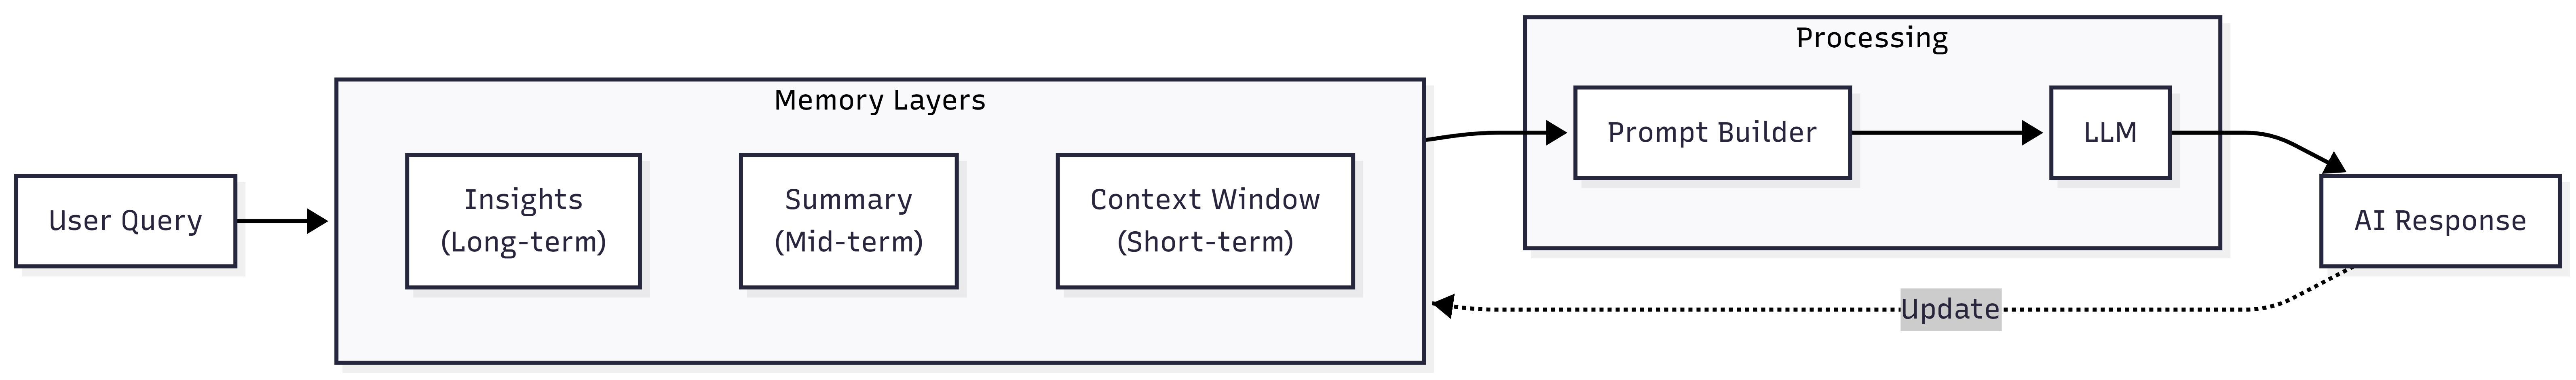
\includegraphics[width=1.0\textwidth]{figure1.png}
\end{center}
\caption{System architecture showing the three-layer memory structure. User queries trigger parallel retrieval from Insights (long-term), Summary (mid-term), and Context Window (short-term), which are combined into a prompt for the LLM.}
\label{fig:architecture}
\end{figure}

\begin{figure}[H]
\begin{center}
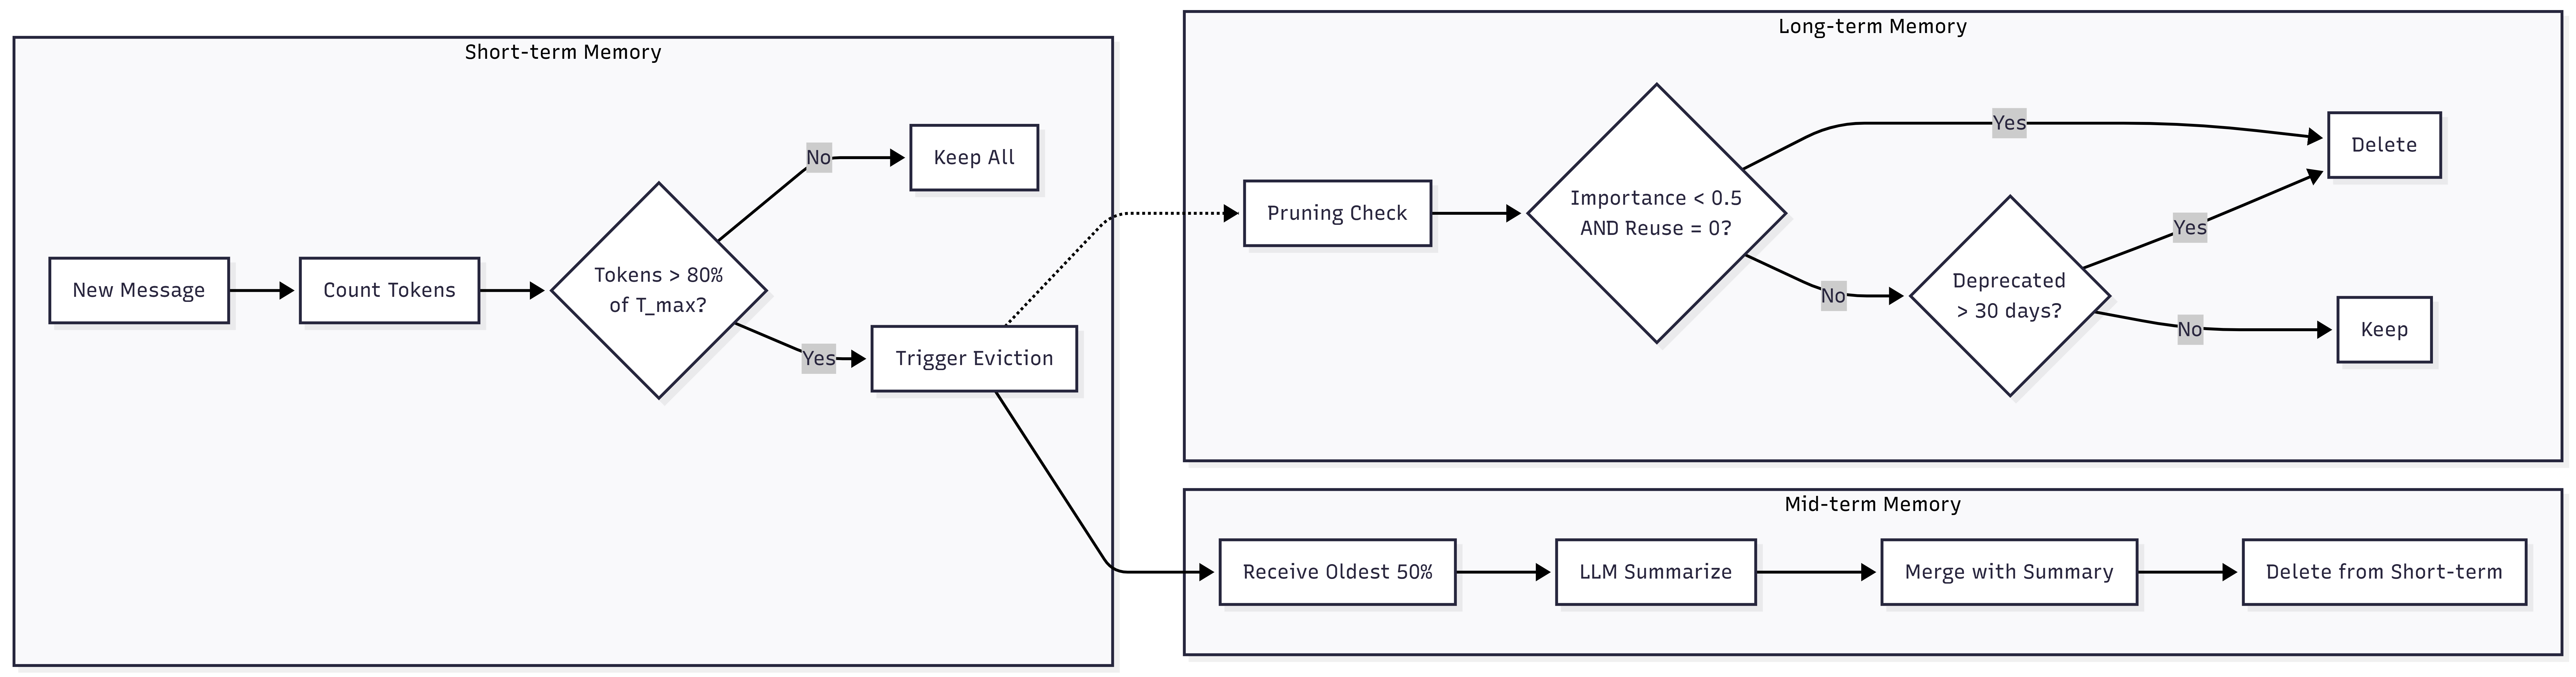
\includegraphics[width=0.8\textwidth]{figure2.png}
\end{center}
\caption{Memory forgetting mechanisms across the three layers. Short-term memory triggers eviction at 80\% capacity, mid-term memory compresses via summarization before deletion, and long-term memory employs intelligent pruning based on importance and deprecation status.}
\label{fig:forgetting}
\end{figure}

\section{Experiments}
\label{sec:experiments}

This section presents two experiments designed to evaluate the proposed memory system: (1) a comparison experiment measuring overall memory retention against a baseline, and (2) an ablation study examining the contribution of individual components.

\subsection{Experimental Setup}
\label{sec:setup}

\textbf{Model Configuration.} All experiments use Qwen3-8B as the underlying LLM, accessed via the SiliconFlow API. The model's context window is 128k tokens, with token allocations as specified in Table~\ref{tab:token_allocation}.

\textbf{Test Protocol.} Each experiment follows a three-phase protocol designed to stress-test long-term memory:
\begin{enumerate}
    \item \textbf{Information Establishment} (5 rounds): The user provides core personal information including name, location, project details, and technical preferences.
    \item \textbf{Context Filling} (10--40 rounds): General technical discussions are conducted to fill the context window and push early information beyond the sliding window boundary.
    \item \textbf{Memory Recall} (5 rounds): Specific questions test whether the system can recall information from Phase 1.
\end{enumerate}

\textbf{Evaluation Metrics.} Memory performance is measured by \textit{keyword recall rate}: the percentage of expected keywords (e.g., user's name, project framework) that appear in the system's responses during Phase 3.

\subsection{Comparison Experiment}
\label{sec:comparison}

The comparison experiment evaluates the full memory system against a baseline that uses only a token-based sliding window (no Summary, no Insights).

\textbf{Setup.} Both systems operate under identical conditions with 2,000 tokens allocated for context---a deliberately constrained budget to ensure that Phase 1 information is evicted from the sliding window during Phase 2. The test consists of 20 rounds following the three-phase protocol (5 + 10 + 5).

\textbf{Results.} Table~\ref{tab:comparison_results} summarizes the comparison results.

\begin{table}[H]
\caption{Comparison experiment results: Baseline vs Full Memory}
\label{tab:comparison_results}
\begin{center}
\begin{tabular}{lccc}
\toprule
\textbf{Metric} & \textbf{Baseline} & \textbf{Full Memory} & \textbf{Change} \\
\midrule
Memory Recall Rate & 33.3\% & 73.3\% & +40.0\% \\
Avg. Response Time & 42.1s & 37.0s & -12.1\% \\
Avg. Response Length & 2,587 chars & 1,295 chars & -50.0\% \\
Active Insights & 0 & 132 & -- \\
\bottomrule
\end{tabular}
\end{center}
\end{table}

The Full Memory system achieves a 73.3\% keyword recall rate compared to 33.3\% for the baseline, representing a 40\% absolute improvement. Notably, the full system also responds faster (12.1\% reduction) and produces more concise responses (50\% shorter), suggesting that retrieved Insights help the model focus on relevant information rather than generating verbose explanations.

Figure~\ref{fig:context_comparison} illustrates the context size evolution during the experiment. The baseline system's context remains relatively stable within the sliding window limit, while the Full Memory system maintains a larger effective context through the combination of recent messages, compressed summaries, and retrieved Insights.

\begin{figure}[H]
\begin{center}
\includegraphics[width=0.8\textwidth]{figure3.png}
\end{center}
\caption{Context size comparison between Baseline (sliding window only) and Full Memory system over 20 conversation rounds.}
\label{fig:context_comparison}
\end{figure}

\subsection{Ablation Study}
\label{sec:ablation}

To understand the contribution of each memory component, an ablation study systematically disables individual modules while keeping others active.

\textbf{Configurations.}
\begin{itemize}
    \item \textbf{Full-System}: All components enabled (Context Window + Summary + Insights)
    \item \textbf{No-Insights}: Summary enabled, Insights extraction and retrieval disabled
    \item \textbf{No-Summary}: Insights enabled, conversation summarization disabled
\end{itemize}

\textbf{Setup.} Each configuration is tested with 50 rounds (5 + 40 + 5) and a context budget of 4,000 tokens to ensure sufficient context filling that triggers the summarization mechanism.

\textbf{Results.} Table~\ref{tab:ablation_results} presents the ablation study results.

\begin{table}[H]
\caption{Ablation study results: Impact of disabling individual components}
\label{tab:ablation_results}
\begin{center}
\begin{tabular}{lccc}
\toprule
\textbf{Configuration} & \textbf{Recall Rate} & \textbf{Change} & \textbf{Insights Count} \\
\midrule
Full-System & 46.7\% & -- & 372 \\
No-Insights & 20.0\% & -26.7\% & 0 \\
No-Summary & 13.3\% & -33.4\% & 402 \\
\bottomrule
\end{tabular}
\end{center}
\end{table}

\textbf{Analysis.} The results reveal that both components contribute significantly to memory retention:

\begin{itemize}
    \item \textbf{Disabling Insights} reduces recall by 26.7\%, demonstrating that the long-term knowledge extraction mechanism captures information that would otherwise be lost when messages are evicted from the context window.
    \item \textbf{Disabling Summary} causes the largest degradation (-33.4\%), indicating that conversation summarization is the most critical component. Without summaries, information from early conversations is permanently lost once evicted, and even active Insights cannot fully compensate.
\end{itemize}

Interestingly, the No-Summary configuration generates slightly more Insights (402 vs 372), likely because the Curator processes more raw conversation content without the compression provided by summaries. However, this does not translate to better recall, confirming that Insights alone cannot replace the contextual continuity provided by summaries.

\subsection{Discussion}
\label{sec:discussion}

The experimental results support three key conclusions:

\textbf{Finding 1: Multi-layer memory significantly outperforms sliding window baselines.} The 40\% improvement in recall rate (33.3\% → 73.3\%) demonstrates that the proposed system effectively addresses the stateless limitation of LLMs for conversational applications.

\textbf{Finding 2: Summary and Insights provide complementary benefits.} The ablation study shows that disabling either component degrades performance, but Summary has a larger impact (-33.4\% vs -26.7\%). This suggests that maintaining narrative continuity through summarization is essential, while Insights provide additional precision for specific knowledge retrieval.

\textbf{Finding 3: Memory augmentation does not increase response latency.} Contrary to expectations, the Full Memory system responds 12.1\% faster than the baseline. This may be attributed to retrieved Insights providing focused context that reduces the model's need to generate lengthy exploratory responses.

\textbf{Limitations.} Several limitations should be noted: (1) the keyword-based recall metric may not capture semantic equivalence or paraphrasing; (2) experiments were conducted with a single LLM (Qwen3-8B), and generalization to other models requires further validation; (3) test cases focused on technical conversations, and performance in other domains may vary.

\section{Conclusion}
\label{sec:conclusion}

This paper presented a multi-layer memory system designed to address the stateless nature of Large Language Models in conversational applications. The proposed architecture combines three complementary mechanisms: a token-based context window for short-term memory, conversation summarization for mid-term memory compression, and a Dynamic Cheatsheet-inspired Insights module for long-term knowledge retention.

Experimental evaluation demonstrates significant improvements over baseline approaches. The comparison experiment shows a 40\% absolute improvement in memory recall rate (33.3\% → 73.3\%) compared to a sliding window baseline. The ablation study reveals that conversation summarization is the most critical component (-33.4\% when disabled), while the Insights module provides substantial complementary benefits (-26.7\% when disabled).

The system operates entirely through standard LLM API calls, requiring no model modifications or fine-tuning, making it readily applicable to existing applications. Future work may explore adaptive token allocation strategies, cross-session memory persistence, and integration with retrieval-augmented generation for external knowledge sources.

\subsubsection*{Acknowledgments}
% TODO: Acknowledgments (optional)


\bibliography{iclr2025_conference}
\bibliographystyle{iclr2025_conference}

\appendix
\section{Appendix}
% TODO: Additional materials (optional)


\end{document}
